\chapter{Questionário para avaliação de soft skills do programador}
\label{ap:tipi}

Você está prestes a responder um questionário que trata de personalidade e está voltado ao seu perfil como programador de software.
Para começar, informe corretamente seu username e email no Huxley: 

\begin{tabular}{lp{5cm}}
Username no Huxley & \noindent\rule{5cm}{0.4pt} \\

Email no Huxley	 	 & \noindent\rule{5cm}{0.4pt} \\
\end{tabular}

\section{Contextualização}

Quando responder o questionário Ten-Item Personality Inventory - TIPI, imagine você mesmo quando está programando, ou seja, avalie seu comportamento em atividades relacionadas à programação. Observe que algumas questões contam com uma breve descrição que te ajudará a contextualizá-las. Seja sincero em suas respostas.

Se desejar consultar o questionário TIPI original (em inglês), veja a página 22 do artigo de Gosling et al. (2003)\nocite{gosling:03}, em:
\href{http://goo.gl/ha6Zr4}{\textsl{http://goo.gl/ha6Zr4}}.

As respostas deste questionário contribuem para a pesquisa de mestrado da aluna Maria Helynne Lima Silva, sob orientação do professor Rodrigo de Barros Paes, do Programa de Pós-Graduação em Informática do Instituto de Computação da Universidade Federal de Alagoas.

\section{Ten-Item Personality Inventory – TIPI}

Aqui estão alguns traços de personalidade que podem ou não aplicar-se a você.  Por favor, escolha um número em cada declaração para indicar o quanto você concorda ou discorda com cada declaração. Você deve pontuar o quanto cada traço aplica-se a você, mesmo se uma característica aplica-se mais fortemente que a outra.

\vspace{0.5cm}
\noindent
\begin{tabular}{lll}
\footnotesize 1 – Discordo fortemente 		& 																						& \footnotesize 5 – Concordo um pouco\\
\footnotesize 2 – Discordo moderadamente 	& \footnotesize 4 – Nem concordo nem discordo	& \footnotesize 6 – Concordo moderadamente\\
\footnotesize 3 – Discordo um pouco 			&																							& \footnotesize 7 – Concordo fortemente\\
\end{tabular}

\vspace{0.5cm}
\textbf{Eu vejo a mim mesmo como:}
\vspace{0.5cm}

\noindent
\textbf{1. Extrovertido, entusiasmado} \footnotesize \textsl{- Em relação a ser comunicativo}
\normalsize
 
\begin{figure}[!h]
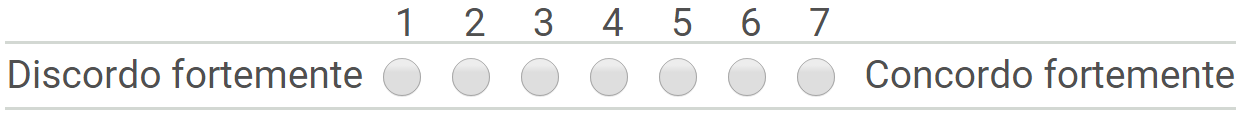
\includegraphics[width=.65\textwidth]{likert.png}
\end{figure}

\newpage%
\noindent
\textbf{2. Crítico, briguento}

\begin{figure}[!h]
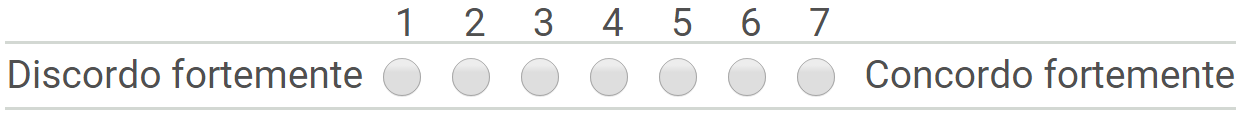
\includegraphics[width=.65\textwidth]{likert.png}
\end{figure}

\noindent  
\textbf{3. Seguro, autodisciplinado}   \footnotesize \textsl{- Em relação a executar suas tarefas com persistência}
\normalsize

\begin{figure}[!h]
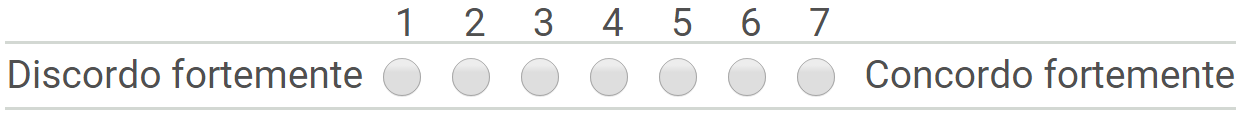
\includegraphics[width=.65\textwidth]{likert.png}
\end{figure}
 
\noindent
\textbf{4. Ansioso, facilmente chateado}

\begin{figure}[!h]
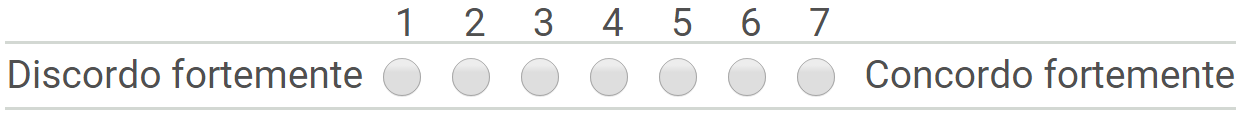
\includegraphics[width=.65\textwidth]{likert.png}
\end{figure}

\noindent
\textbf{5. Aberto a novas experiências, complexo} 

\begin{figure}[!h]
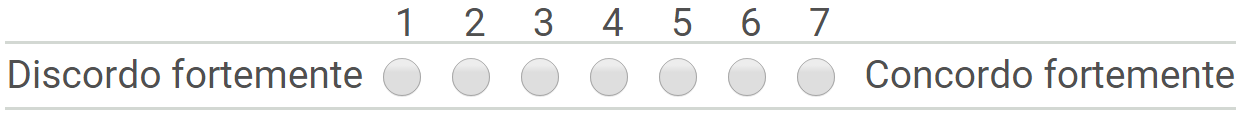
\includegraphics[width=.65\textwidth]{likert.png}
\end{figure}
 
\noindent
\textbf{6. Reservado, quieto}          \footnotesize \textsl{- Em relação a pedir ajuda de outras pessoas} \normalsize

\begin{figure}[!h]
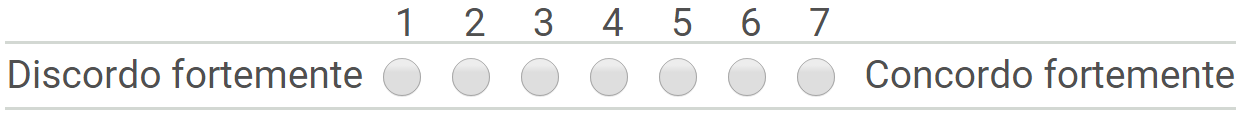
\includegraphics[width=.65\textwidth]{likert.png}
\end{figure}
 
\noindent
\textbf{7. Compreensivo, amável}       \footnotesize \textsl{- Em relação à forma como lida com as pessoas}\normalsize

\begin{figure}[!h]
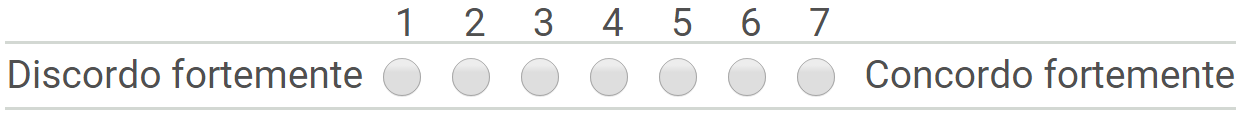
\includegraphics[width=.65\textwidth]{likert.png}
\end{figure}

\noindent
\textbf{8. Desorganizado, descuidado}

\begin{figure}[!h]
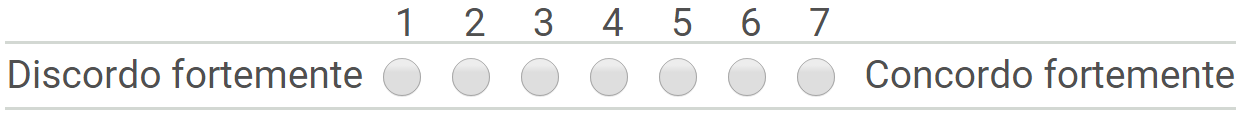
\includegraphics[width=.65\textwidth]{likert.png}
\end{figure}
 
\noindent
\textbf{9. Calmo, emocionalmente estável}

\begin{figure}[!h]
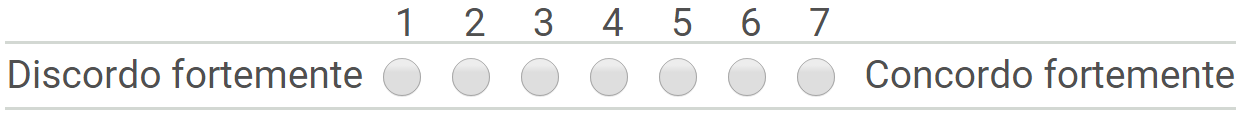
\includegraphics[width=.65\textwidth]{likert.png}
\end{figure}
 
\noindent
\textbf{10. Convencional, não criativo}  

\begin{figure}[!h]
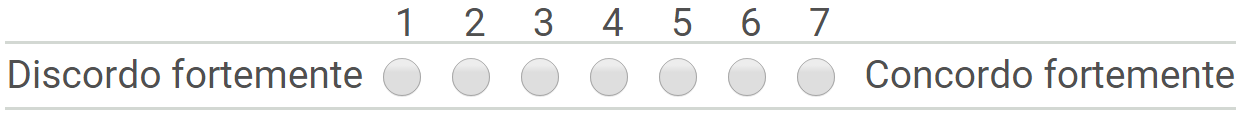
\includegraphics[width=.65\textwidth]{likert.png}
\end{figure}

